% file thesis.tex
% Archivo thesis.tex
% Documento maestro que incluye todos los paquetes necesarios para el documento
% principal.

% Documento obtenido por un sinfin de iteraciones de administradores del LDC
% Estructura actual hecha por:
% Jairo Lopez <jairo@ldc.usb.ve>
% Actualizado ligeramente por:
% Alexander Tough 

\documentclass[oneside,12pt,letterpaper]{report}
\tolerance=1000  
\hbadness=10000  
\raggedbottom

% Para escribir algoritmos
\usepackage{listings}
\usepackage{algpseudocode}
\usepackage{algorithmicx}
\usepackage{algorithm}

% Paquetes para manejar graficos
\usepackage{epsf}
\usepackage[pdftex]{graphicx}
\usepackage{epsfig}
% Simbolos matematicos
\usepackage{latexsym,amssymb}
% Paquetes para presentar una tesis decente.
\usepackage{setspace,cite} % Doble espacio para texto, espacio singular para
                           % los caption y pie de pagina
\usepackage[table]{xcolor}
\usepackage{tikz}
\usetikzlibrary{shapes.geometric,arrows}

\usetikzlibrary{arrows,shapes}
\usepackage{verbatim}

\usepackage{comment}

% Paquetes no utilizados para citas
%\usepackage{mcite} 
%\usepackage{draft} 

\usepackage{wrapfig}
\usepackage{alltt}

% Acentos 
\usepackage[spanish,activeacute,es-noquoting]{babel}

\usepackage[spanish]{translator}
\usepackage[utf8]{inputenc}
\usepackage{color, xcolor, colortbl}
\usepackage{multirow}
\usepackage{subfig}
\usepackage[OT1]{fontenc}
\usepackage{tocbibind}
\usepackage{anysize}
\usepackage{listings} 

% Para poder tener texto asiatico
%\usepackage{CJK}

% Opciones para los glosarios
\usepackage[style=altlist,toc,numberline,acronym]{glossaries}
\usepackage{url}
\usepackage{amsthm}
\usepackage{amsmath}
\usepackage{fancyhdr} % Necesario para los encabezados
\usepackage{fancyvrb}
\usepackage{makeidx} % En caso de necesitar indices.
\makeindex  % Necesitado para los indices

% Definiciones para definicions, teoremas y lemas
\theoremstyle{definition} \newtheorem{definicion}{Definici\'{o}n}
\theoremstyle{plain} \newtheorem{teorema}{Teorema}
\theoremstyle{plain} \newtheorem{lema}{Lema}

% Para la creacion de los pdfs
\usepackage{hyperref}

% Para resolver el lio del Unicode para la informacion de los PDFs
% En pdftitle coloca el nombre de su proyecto de grado/pasantia.
% En pdfauthor coloca su nombre.
\hypersetup{
    pdftitle = {Desarrollo de una aplicación móvil basada en el sistema operativo AndroidOS para el portal Tuguia.de},
    pdfauthor={Juan Rosas},
    colorlinks,
    citecolor=black,
    filecolor=black,
    linkcolor=black,
    urlcolor=black,
    backref,
    pdftex
}

\definecolor{brown}{rgb}{0.7,0.2,0}
\definecolor{darkgreen}{rgb}{0,0.6,0.1}
\definecolor{darkgrey}{rgb}{0.4,0.4,0.4}
\definecolor{lightgrey}{rgb}{0.95,0.95,0.95}

\usepackage{listings}
\lstnewenvironment{code}{\lstset{basicstyle=\small}}{}

\lstset{escapeinside=~~}
\lstset{
   frame=single,
   framerule=1pt,
   showstringspaces=false,
   basicstyle=\footnotesize\ttfamily,
   keywordstyle=\textbf,
   backgroundcolor=\color{lightgrey}
}

% Crea el glosario
\makeglossaries

% Incluye el glosario
%\input{apendices/glosario.tex}

% Para crear la hoja escaneada de las firmas
\usepackage[absolute]{textpos}

% Pone los nombres y las opciones para mostrar los codigos fuentes
\lstset{language=java, breaklines=true, frame=single, showstringspaces=false,
        showtabs=false, numbers=left, keywordstyle=\color{black},
        basicstyle=\footnotesize, captionpos=b }
\renewcommand{\lstlistingname}{C\'{o}digo fuente}
\renewcommand{\lstlistlistingname}{\'{I}ndice de c\'{o}digos fuentes}

\newcommand{\todo}{ TODO: }

% Dimensiones de la pagina
\setlength{\headheight}{15pt}
\marginsize{3cm}{2cm}{2cm}{2cm}

%%%%%%%%%%%%%%%%%%%%%%%%%%%%%%%%%%%%%%%%%%%%%%%%%%%%%%%%%%%%%%%%%%%%%%%%%%%
%%%%%%%%%%%%%%%%      end of preamble and start of document     %%%%%%%%%%%
%%%%%%%%%%%%%%%%%%%%%%%%%%%%%%%%%%%%%%%%%%%%%%%%%%%%%%%%%%%%%%%%%%%%%%%%%%%
\begin{document}

% Pagina de titulo
% Pagina de titulo
\begin{titlepage}
\begin{center}

% Upper part (aqui ya esta incluido el logo de la USB).

\includegraphics[scale=0.5,type=png,ext=.png,read=.png]{imagenes/cebolla} \\

% Encabezado
\textsc {\large UNIVERSIDAD SIMÓN BOLÍVAR} \\
\textsc{\bfseries DECANATO DE ESTUDIOS PROFESIONALES\\
COORDINACI'ON DE INGENIER'IA DE LA COMPUTACI'ON}

\bigskip
\bigskip
\bigskip
\bigskip
\bigskip
\bigskip
\bigskip
\bigskip
\bigskip

% Title/Titulo
% Aqui ponga el nombre de su proyecto de grado/pasantia larga
\textsc{\bfseries Desarrollo de una aplicación móvil basada en el sistema operativo AndroidOS para el portal Tuguia.de}

\bigskip
\bigskip
\bigskip
\bigskip
\bigskip

% Author and supervisor/Autor y tutor
\begin{minipage}{\textwidth}
\centering
Por: \\
Juan Vicente Rosas Ramirez 

\bigskip
\bigskip
\bigskip

Realizado con la asesor'ia de: \\
Tutor Académico: Carmen Rosseline Rodríguez \\
Tutor Industrial: Gianpaolo Valero
\end{minipage}

\bigskip
\bigskip
\bigskip
\bigskip
\bigskip
\bigskip
\bigskip
\bigskip
\bigskip

% Bottom half
{PROYECTO DE PASANTÍA LARGA \\ Presentado ante la Ilustre Universidad Sim'on Bol'ivar \\
como requisito parcial para optar al t'itulo de \\ Ingeniero en Computaci'on} \\

\bigskip
\bigskip
\vfill

% Date/Fecha 
{\large \bfseries Sartenejas, 
%FECHA
Septiembre de 2013}

\end{center}
\end{titlepage}


% Pagina de acta final (vacio)
%% Pagina del acta final
\begin{titlepage}
\begin{center}

% Upper part

\includegraphics[scale=0.5,type=png,ext=.png,read=.png]{imagenes/cebolla} \\

\textsc {\large UNIVERSIDAD SIM'ON BOL'IVAR} \\
\textsc{DECANATO DE ESTUDIOS PROFESIONALES\\
COORDINACI'ON DE INGENIER'IA DE LA COMPUTACI'ON}

\bigskip
\bigskip
\bigskip
\bigskip
\bigskip
\bigskip

% Title
\textsc{ACTA FINAL PASANT\'IA LARGA}

\bigskip
\bigskip

% Aqui coloca el nombre de su proyecto de grado/pasantia larga.
\textsc{\bfseries Desarrollo de una aplicación móvil basada en el sistema operativo AndroidOS para el portal Tuguia.de}

\bigskip
\bigskip
\bigskip
\bigskip

\begin{minipage}{\textwidth}
\centering
Presentado por: \\
% Aqui coloca su nombre.
\textsc{\bfseries Juan Vicente Rosas Ramirez} \\

\bigskip
\bigskip
\bigskip
\bigskip

Esta Pasant\'ia Larga ha sido aprobado por el siguiente jurado examinador: \\

\bigskip
\bigskip

% Despues de cada line coloca el (los) nombre(s) de
% cada uno de los integrantes del jurado.
\line(1,0){200} \\
Prof. Rosseline Rodríguez\\

\bigskip
\bigskip

\line(1,0){200} \\
PROFESOR 2 \\

\bigskip
\bigskip

\line(1,0){200} \\
Ing. Gianpaolo Valero \\
\end{minipage}

\bigskip
\bigskip
\vfill

% Date/Fecha
{\large \bfseries Sartenejas, 23/09/2013 }

\end{center}
\end{titlepage}

%\includegraphics[width=\textwidth, height=\textheight]{figures/acta.jpg}

\setcounter{secnumdepth}{4}
\setcounter{tocdepth}{4}

% Define encabezado numeros romanos y como se separan los captiulos y las
% secciones
\addtolength{\headheight}{3pt}
\pagenumbering{roman}
\pagestyle{fancyplain}

\renewcommand{\chaptermark}[1]{\markboth{\chaptername\ \thechapter:\,\ #1}{}}
\renewcommand{\sectionmark}[1]{\markright{\thesection\,\ #1}}

\onehalfspacing

\lhead{}
\chead{}
\rhead{}
\renewcommand{\headrulewidth}{0.0pt}
\lfoot{}
\cfoot{\fancyplain{}{\thepage}}
\rfoot{}

% Pagina de resumen
% Pagina del acta final
\begin{titlepage}
\begin{center}

% Upper part

\includegraphics[scale=0.5,type=png,ext=.png,read=.png]{imagenes/cebolla} \\

\textsc {\large UNIVERSIDAD SIM'ON BOL'IVAR} \\
\textsc{DECANATO DE ESTUDIOS PROFESIONALES\\
COORDINACI'ON DE INGENIER'IA DE LA COMPUTACI'ON}

\bigskip
\bigskip
\bigskip
\bigskip
\bigskip
\bigskip

% Title
\textsc{ACTA FINAL PASANT\'IA LARGA}

\bigskip
\bigskip

% Aqui coloca el nombre de su proyecto de grado/pasantia larga.
\textsc{\bfseries Desarrollo de una aplicación móvil basada en el sistema operativo AndroidOS para el portal Tuguia.de}

\bigskip
\bigskip
\bigskip
\bigskip

\begin{minipage}{\textwidth}
\centering
Presentado por: \\
% Aqui coloca su nombre.
\textsc{\bfseries Juan Vicente Rosas Ramirez} \\

\bigskip
\bigskip
\bigskip
\bigskip

Esta Pasant\'ia Larga ha sido aprobado por el siguiente jurado examinador: \\

\bigskip
\bigskip

% Despues de cada line coloca el (los) nombre(s) de
% cada uno de los integrantes del jurado.
\line(1,0){200} \\
Prof. Rosseline Rodríguez\\

\bigskip
\bigskip

\line(1,0){200} \\
PROFESOR 2 \\

\bigskip
\bigskip

\line(1,0){200} \\
Ing. Gianpaolo Valero \\
\end{minipage}

\bigskip
\bigskip
\vfill

% Date/Fecha
{\large \bfseries Sartenejas, 23/09/2013 }

\end{center}
\end{titlepage}


% Pagina de resumen
\setcounter{page}{4}
\pdfbookmark[0]{Resumen}{resumen} % Sets a PDF bookmark for the dedication
\begin{center}
	{\bf Resumen}
\end{center}	

Empresas TD es una empresa dedicada a ofrecer soluciones tecnológicas e innovadoras orientadas a mejorar la calidad del e-commerce en Venezuela y a brindar la oportunidad de darse a conocer a los diferentes comercios y locales de las principales ciudades del país en este medio.

Bajo este precepto Empresas TD crea el portal Tuguia.De con el objetivo de convertirse en la 
principal guía de locales y comercios del país. Dado el crecimiento de Tuguia.De como proyecto, la empresa decide llevar esta idea a las plataformas móviles comenzando con el desarrollo de una aplicación nativa para el sistema operativo AndroidOs. 

Este informe describe las actividades realizadas durante el desarrollo del proyecto de pasantía larga, que consistió en la elaboración de una aplicación móvil para el portal Tuguia.de. Dicha aplicación permite llevar la iniciativa de este portal a un mayor número de usuarios de una forma sencilla, permitiendo así que éstos puedan acceder a los diferentes servicios prestados por esta guía desde cualquier lugar usando su teléfono celular Android.

El desarrollo de esta aplicación móvil, se realizó siguiendo el proceso iterativo e incremental de la metodología ágil Scrum, y los principios del desarrollo guiado por 
pruebas y comportamientos (\textit{test-driven development y behavior-driven development}). 
Fue realizada con el lenguaje de programación \textit{Java}, haciendo uso del entorno de trabajo dispuesto para Android (\textit{Android SDK}) y SQLite como manejador de base de datos de la aplicación en el dispositivo.

Como resultado de este proyecto de pasantía se realizó el análisis, diseño e implementación de la aplicación móvil que cubre los requerimientos planteados en el alcance inicial. Adicionalmente se realizó la configuración de un servidor de ApacheSolr para mejorar
el resultado de las búsquedas y diversas mejoras funcionales al API (\textit{Aplication Programming Interface}) que permite acceder a las funcionalidades del portal Tuguia.De siendo 
éste la materia prima de la aplicación móvil.



% Pagina de dedicatoria (opcional)
\pagebreak

\setcounter{page}{5}

\vspace*{8cm} 
\pdfbookmark[0]{Dedicatoria}{dedicatoria} % Sets a PDF bookmark for the dedication
\begin{center} 
\large A Dios, mi familia, profesores y amigos.
\end{center}
\newpage


% Pagina de agradecimientos (opcional)
\setcounter{page}{6}

\chapter*{Agradecimientos
\markboth{Agradecimientos}{Agradecimientos}}

El presente 

\bigskip
En primer lugar 


% Crea la tabla de contenidos
\tableofcontents

% Crea la lista de cuadros
%\listoftables

% Crea la lista de figuras
%\listoffigures

% Crea la lista de codigos fuentes
%\lstlistoflistings

\clearpage

% Define encabezado en numeros arabicos  
\pagenumbering{arabic}

\fancyhf{} % Redefine el encabezado 
\lhead{}
\chead{}
\rhead{\fancyplain{}{\thepage}}
\renewcommand{\headrulewidth}{0.0pt}
\lfoot{}
\cfoot{}
\rfoot{}

\doublespacing

% Incluye los archivos deseados - El contenido de su proyecto de grado/pasantia larga.
\chapter*{Introducción}

\pdfbookmark[0]{Introducción}{introducion} % Sets a PDF bookmark for the dedication

\label{sect:justificacion}

\label{sect:planteamiento}

\label{sect:objetivos}


% Marco Teorico.
\chapter{Entorno Empresarial} \label{chap:entorno}

\vspace{5 mm}

En este capítulo se realizará una descripción de Empresas TD y sus antecedentes, ademas se explicará en que consiste el portal web Tuguia.de que se tiene planteado logre convertirse en el núcleo de negocio para Empresas TD, así como el resto de su portafolio de productos y de esta forma dar a conocer el entorno laboral en el que se realizó el proyecto de pasantía.

  
\section{Antecedentes de la Empresa} \label{sect:Antecedentes_empresa}

En el año 2010 la compañía Servicios 1488 C.A. realizó el lanzamientos del portal Tudescuenton.com, con el objetivo de brindar a todos los venezolanos los mejores 
descuentos en los diferentes comercios asociados, convirtiéndose así en la primera 
empresa de venta de cupones de descuento del país.

El crecimiento de Tudescuenton.com y las nuevas tendencias de comercio electrónico 
llevó a la compañía Servicios 1488 C.A. a consolidarse en lo que hoy se conoce 
como Empresas TD añadiendo a su portafolio de productos diferentes iniciativas 
que le permiten ofrecer soluciones tecnológicas orientadas a mejorar la calidad del 
comercio electrónico en Venezuela y a brindar la oportunidad de darse a conocer a los diferentes comercios y locales de las principales ciudades del país en este medio.

De esta forma surge el portal Tuguia.de con el objetivo de convertirse en la principal 
guía de locales y comercios del país, y en un espacio donde los usuarios puedan compartir 
sus experiencias al visitar estos comercios. Se tiene previsto que Tuguia.de se convierta
en el núcleo del negocio de Empresas TD, ya que este portal permitirá centralizar los
diferentes servicios prestados por la compañía. 



\section{Misión} \label{sect:Mision}
Aquí va la misión de la empresa. 
Aquí va la misión de la empresa. 
Aquí va la misión de la empresa. 
Aquí va la misión de la empresa. 
Aquí va la misión de la empresa. 

\section{Visión} \label{sect:Vision}
Aquí va la Visión de la empresa. 

Pedir a Gianpaolo o Alfredo

\section{Estructura Organizacional} \label{sect:Estructura_organizacional}

Empresas TD es una compañía con una gran proyección a futuro compuesta mayormente 
por gente joven. El perfil buscado en los miembros del equipo de trabajo es el de 
un profesional dinámico, creativo e innovador, comprometido por brindar a los
asociados y usuarios experiencias de alta calidad. 

Actualmente se gestionan 4 proyectos en Empresas TD, como se puede ver en la figura \ref{fig:ogtd}y se describen a continuación:

\begin{figure}[h]
	\begin{center}
		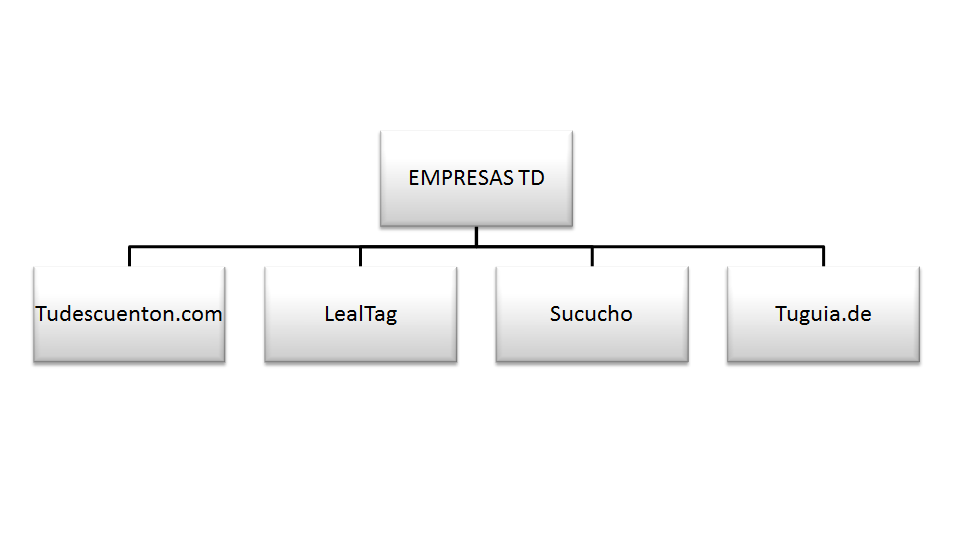
\includegraphics[scale=0.4]{imagenes/OrganigramaTD.png}
	\end{center}
	\caption{
		\label{fig:ogtd}
		Organigrama de Empresas TD.
	}
\end{figure}



\begin{itemize}
  \item \textbf{Tudescuenton:} es el sistema que le brinda a los venezolanos, la oportunidad de conocer las mejores cosas que hacer, en las principales ciudades del país, a través de descuentos insuperables\cite{TDC}.
  \item \textbf{Lealtag:} LealTag es la plataforma que te permite recibir premios, descuentos y regalos en tus sitios favoritos por ser un cliente frecuente\cite{LTG}.
  \item \textbf{Sucucho:} es un portal que ofrece a los creativos venezolanos un espacio en donde pueden exponer su talento ante el país, en el cual brindamos la oportunidad de que cada uno tenga su tiendita propia 365 días al año\cite{SCC}.
  \item \textbf{Tuguiade:} Tuguía.de es una página que sirve para conectar los locales con sus clientes. Ofreciéndoles a los usuarios información verificada de los mismos y la posibilidad de escribir sobre sus experiencias, subir fotos e intercambiar historias con los otros clientes\cite{TGD}. 
\end{itemize}
  
Cada proyecto tiene asignado un director general y un esquema organizacional específico que se ajusta a sus necesidades. En el caso de Tuguia.de; proyecto en el que desarrolló el proyecto de pasantía, el organigrama se muestra en la figura \ref{fig:ogtgd}donde se puede observar la estructura organizativa de la que el pasante fue parte. 

\begin{figure}[h]
	\begin{center}
		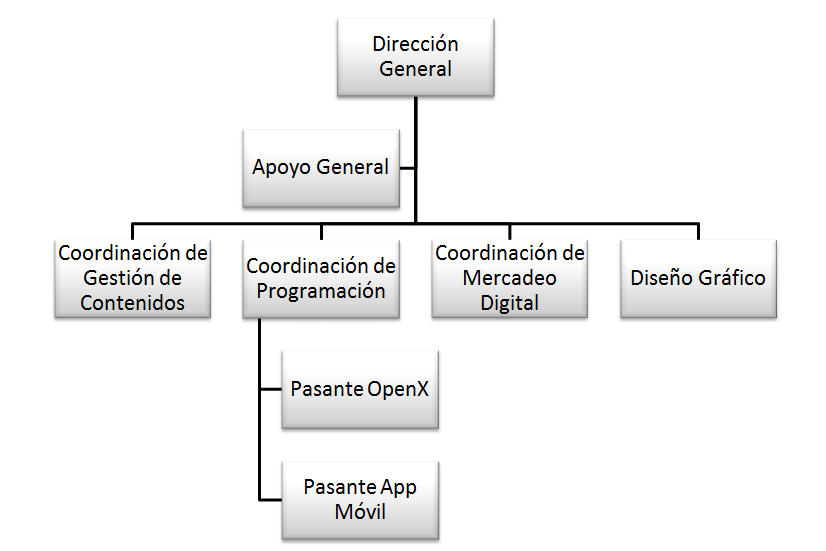
\includegraphics[scale=0.4]{imagenes/OrganigramaTGD.png}
	\end{center}
	\caption{
		\label{fig:ogtgd}
		Organigrama de Tuguia.de
	}
\end{figure}
 
\section{Ubicación del Pasante} \label{sect:ubicacion_pasante}

El proyecto de pasantía llevado a cabo en el periodo Abril-Septiembre de 2013 se
realizó bajo la tutela del Ing. Gianpaolo Valero Gerente del Departamento de Tecnología
de Empresas TD y bajo la supervisión directa del Lic. Alexander Mayora, coordinador de desarrollo del proyecto Tuguia.de. 

Durante el desarrollo el proyecto el pasante fue miembro del equipo de Tecnología de 
Tuguia.de estando ubicado en la oficina correspondiente a este. Para el desarrollo 
le fue asignado un escritorio compartido y un computador personal con acceso a Internet.


%% Defeinición.
\chapter{Definición del Proyecto} \label{chap:definicion_proyecto}

\vspace{5 mm}

A continuación en este capítulo se presentan los motivos que llevaron a la realización de este proyecto de pasantía, se realiza una descripción del problema planteado y la solución propuesta, así como los objetivos tanto generales como específicos definidos al inicio del desarrollo y el alcance del proyecto.
%\section{Motivación y Antecedentes} \label{sect:motivacion}

En la sociedad actual se hace imprescindible que las empresas posean una pagina web; el mundo que hoy conocemos se basa en Internet y es en este donde la gente busca las respuestas a sus inquietudes cotidianas. Actualmente en el mundo existen casi el doble de \textit{smartphones} que computadores personales \cite{DGT} y según los resultados obtenidos en una encuesta realizada por Google en cunjunto con IPSOS OTX mediaCT al final del 2010, aparte de recibir y hacer llamadas, las actividades más realizadas en los teléfonos inteligentes son navegar en Internet, el uso de motores de búsquedas y en tercer lugar el uso de aplicaciones \cite{TMM}. Para las empresas, ya no sólo es necesario estar en la web, deben estar al alcance de los teléfonos inteligentes.

Los \textit{smartphones} han llegado a ser parte de la vida de las personas y son dispositivos mucho mas personales que una computadora portátil o de escritorio, estos teléfonos han penetrado hasta el punto que muchos usuarios raramente se separan de sus equipos móviles durante el día. Tomando en cuenta esto y las proyecciones de negocio de \textit{Tuguia.de}; de ser la principal guía de comercios y locales del país, se hace necesario el desarrollo de un mecanismo para que los usuarios puedan acceder a la información del portal desde sus celulares y así hacer de \textit{Tuguia.de} un servicio 24/7, accesible desde cualquier momento y lugar.

Conscientes de la influencia en el éxito de \textit{Tuguia.de} que puede tener la versión móvil de la guía, se decide emprender un desarrollo que permita llevar la aplicación a los celulares inteligentes, sin embargo, existen varias alternativas a considerar si se desea establecer presencia de un negocio en los dispositivos móviles; aplicaciones nativas, aplicaciones híbridas o multiplataforma y paginas web diseñadas específicamente celulares.

Las aplicaciones nativas, llevan este nombre porque son desarrollos implementados en el lenguaje nativo del dispositivo, gracias a esto, sacan el mejor rendimiento posible del \textit{hardware} del móvil, así que tienen un alto desempeño y permiten acceder a las diferentes características presentes en los teléfonos inteligentes con mayor facilidad, sin embargo, el hecho de necesitar un desarrollo en un lenguaje específico, distinto para cada plataforma eleva los costos y el tiempo de desarrollo. 

Las aplicaciones híbridas permiten escribir código en un solo lenguaje para después exportarlo a código nativo y de esta manera obtener una aplicación que funcione en las múltiples plataformas con un solo desarrollo, es de notar que estas aplicaciones tienen un bajo desempeño si las comparamos con las nativas, ademas en estos entornos multiplataforma se dificulta la tarea de acceder a los diferentes componentes del equipo móvil con efectividad. 

Las páginas web de diseño específico para equipos móviles son sitios web que pueden cambiar la forma en la que muestran su contenido de acuerdo al equipo en el que se esta visualizando y de esta manera aprovechar al máximo las dimensiones de las pantallas de los dispositivos, así se consigue que con un solo desarrollo se obtiene un producto que puede operar en tanto en las computadoras como en equipos móviles, al igual que las otras paginas web éstas se ejecutan en un navegador, por lo que se torna bastante complejo acceder a las características propias de los teléfonos inteligentes de hoy en día. 

Luego de evaluar estas alternativas, la junta directiva de \textit{Tuguia.de} decide que desarrollar una aplicación nativa para su proyecto, a pesar de los costos elevados y los altos tiempos de desarrollo desean que la aplicación sea lo mas extensible posible, no obstante, es necesario determinar cuál sistema operativo móvil es el más adecuado para iniciar las versiones móviles de \textit{Tuguia.de}

Según un estudio realizado para finales del 2012 en los Estados Unidos,\cite{NTD} para el tercer trimestre de ese año la participación de Android en el mercado de teléfonos inteligentes era del 52\%, los resultados de dicho estudió lo podemos observar en la figura \ref{fig:marketshare}.
   
\begin{figure}[h]
	\begin{center}
		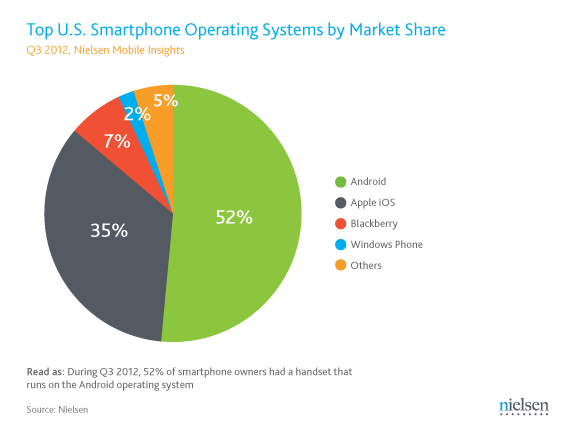
\includegraphics[scale=0.5]{imagenes/Q3-2012-US-Smartphone-OS-market-share.png}
	\end{center}
	\caption{
		\label{fig:marketshare}
		Participación de mercado por sistema operativo móvil \cite{NTD}
	}
\end{figure}

Se hace notable la superioridad de Android sobre los demás sistemas operativos, por lo que es el sistema escogido para iniciar el desarrollo móvil de \textit{Tuguia.de}, pensado en un futuro a corto plazo expandirse al iOS de Apple.

%\section{Planteamiento del Problema y Solución Propuesta} \label{sect:planteamiento_solucion}

Actualmente \textit{Tuguia.de} cuenta con funcionalidades tales como búsqueda de locales dadas sus ubicación y/o una serie de taxonomías asociadas a éstos, además siempre que se muestra información de un local se debe mostrar su ubicación en el mapa, dirección, fotografías asociadas e información de contacto. Un aspecto importante para la visión de negocio de \textit{Tuguia.de} es la capacidad de que los usuarios puedan realizar comentarios y establecer una puntuación de uno a cinco  sobre los locales, esto con el objetivo de brindar no solo la información básica de un establecimiento, sino también priorizar los locales de acuerdo a la opinión de los usuarios. Adicionalmente, \textit{Tuguia.de} prevé ofrecer la posibilidad a los dueños de cada local de gestionar la información de su comercio y campañas de publicidad en el sitio.

El Proyecto de pasantía consiste en llevar las funcionalidades presentes a una aplicación móvil para el sistema operativo Android, agregando nuevas funcionalidades aprovechando los elementos propios de los teléfonos inteligentes como geolocalización y así realizar búsquedas usando la posición actual del equipo y de esta forma brindar información más precisa a los usuarios de \textit{Tuguia.de}.

Para exportar la funcionalidad de \textit{Tuguia.de} se desarrolló un API (Aplication Programming Interface), que permite gestionar el contenido de la página a través de él. La aplicación móvil debe usar este API como materia prima para realizar sus operaciones y de esta manera mantener comunicación constante con la aplicación de \textit{Tuguia.de} para mantener el contenido siempre actualizado.

La figura \ref{fig:AndroidVersion} muestra la distribución de equipos por sistema operativo.  

\begin{figure}[h]
	\begin{center}
		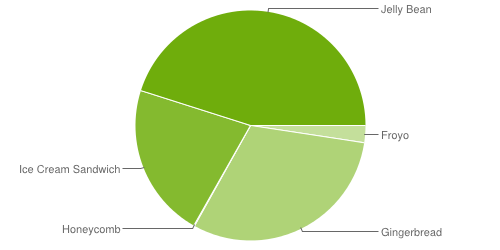
\includegraphics[scale=0.5]{imagenes/chart.png}
	\end{center}
	\caption{
		\label{fig:AndroidVersion}
		Distribución de dispositivos Android por sistemas operativos.
	}
\end{figure}

Se espera que la aplicación móvil, pueda operar efectivamente en las diferentes versiones activas de Android, al menos en las que concentran la mayor cantidad de usuarios. Además debe tener un uso mínimo de la red de datos y poseer una interfaz sencilla y fácil de usar.


%\section{Objetivo General} \label{sect:objetivo_general}

El proyecto de pasantía larga tiene como objetivo general: \textbf{Desarrollar una aplicación móvil basada en el sistema operativo AndroidOS para el portal Tuguia.de}, que permita realizar búsquedas avanzadas sobre los locales, mostrar la información detallada de un local, realizar comentarios y que posea un manejo básico de usuarios.

 
%\section{Objetivos Específicos} \label{sect:objetivos_especificos}

\begin{itemize}
\item Estudiar la arquitectura de la plataforma de desarrollo de Android, entornos de pruebas y demás tecnologías asociadas.
\item Diseñar y desarrollar un mecanismo de comunicación con el API de \textit{Tuguide.de}.
\item Realizar los ajustes y extensiones necesarias sobre el API de \textit{Tuguide.de} para garantizar el funcionamiento deseado.
\item Diseñar e implementar un modelo de datos que permita gestionar los diferentes nodos de información presentes en \textit{Tuguide.de} dentro la aplicación móvil. 
\item Desarrollar un modulo que permita realizar búsquedas avanzadas, usando palabras claves y una ubicación que puede ser coordenadas geográficas o el nombre de un lugar.
\item Diseñar y desarrollar un componente que permita visualizar los locales de \textit{Tuguide.de} en la aplicación móvil.  
\item Diseñar e implementar la funcionalidad que permita subir comentarios asociados a un local de \textit{Tuguide.de}.
\item Implementar diferentes mecanismos que permitan que la aplicación genere la menor transmisión de datos vía red celular posible.

\end{itemize}
%\section{Alcance} \label{sect:alcance}

El presente proyecto pretende generar una versión beta de la aplicación móvil de \textit{Tuguia.de} en la plataforma Android; de manera que esta sea estable y se encuentre en un estado de completitud suficiente para ser aprobada por la directiva de la empresa y pasar a una fase de prueba mas extensa pre-despliegue. 

% Marco Teorico.
\chapter{Marco teórico} \label{chap:marco_teorico}

\vspace{5 mm}

En este capítulo se presentan los fundamentos teóricos más relevantes involucrados en el desarrollo de la pasantía, así como las herramientas y tecnologías utilizadas en el proyecto.
\section{Aspectos del Negocio} \label{sect:aspectos_negocio}
  
Al consistir el proyecto de pasantía en el desarrollo de la versión móvil para el portal Tuguia.de, se hace necesario comprender algunos de los conceptos y términos asociados con el negocio y de esta manera facilitar el entendimiento de los posteriores capítulos.

\subsection{Local} \label{subsect:local}

Un local comercial es un establecimiento que tiene como objetivo principal el desarrollo de alguna actividad comercial o económica. Los locales pueden ofrecer productos o servicios. Algunos ejemplos para los primeros son supermercados, farmacias, tiendas, etc. En el caso de los locales que ofrecen servicios podemos mencionar restaurantes, lugares de entretenimiento como cines o discotecas, entre otros.\cite{DLC}


\subsection{Taxonomías} \label{subsect:taxonomia}

Una taxonomía es un tipo de vocabulario o conjunto de palabras en que todos los términos están conectados, su objetivo es organizar la información y mejorar la búsqueda de contenidos en los sitios web \cite{CM05}. En el caso de Tuguia.de las taxonomías usadas son: 
ciudad, urbanización, categoría, subcategoría y atributos.

\subsection{Reseña} \label{subsect:resena}

``Para Tuguía.de, una reseña es un pequeño texto en donde el usuario cuenta su experiencia.  Puede ser también llamada comentario. Éstas serán escritas en los cuadros de texto dentro de cada local, y servirán para que cada usuario cuente su historia''\cite{TGD}. Para que una reseña sea válida el usuario debe asignarle una calificación de uno a cinco al local que esta comentando.

 



\section{Aspectos Tecnológicos} \label{sect:aspectos_tecnologicos}

En esta sección se presentan las tecnologías y herramientas utilizadas en el desarrollo de la pasantía, así como también algunos términos asociados que son de obligatoria referencia para facilitar al lector la comprensión del contenido subsiguiente. Es necesario hacer una separación entre las tecnologías y herramientas utilizadas para el desarrollo de la aplicación móvil y las asociadas a Tuguia.de con las que se interactuó en el transcurso de la pasantía.

\subsection{Tecnologías Asociadas con la Aplicación Móvil} \label{subsect:Asociadas_movil}

A continuación se presentan las diferentes tecnologías y herramientas involucradas en la construcción de la aplicación Android para Tuguia.de 

\subsubsection{Teléfono Inteligente}

Los teléfonos inteligentes o \textit{smartphones}, son teléfonos celulares que ademas de poseer las características habituales de un celular común, permiten acceder a una series de aplicaciones integradas, navegar en Internet, tomar fotografías, grabar vídeos, entre otras funcionalidades que lo asemejan  a una computadora portátil móvil \cite{PCM}. El objetivo del proyecto de pasantía es llevar a Tuguia.de a estos dispositivos.

\subsubsection{Android}

Android es un sistema operativo basado en \textit{Linux}, diseñado en principio para dispositivos móviles con pantalla táctil, es de código abierto y es liberado bajo la licencia Apache; una licencia bastante flexible, que permite que cualquier desarrollador realice aplicaciones y las integre al sistema sin dificultad.

Las aplicaciones nativas se desarrollan, usando el SDK (\textit{Software Development Kit}) y escribiendo la aplicación en lenguaje \textit{Java}. El SDK es un paquete proporcionado directamente por Google que encapsula todas las bibliotecas y herramientas de desarrollo necesarias para crear, probar, y depurar las aplicaciones \cite{ASDK}. Por otro lado existe la alternativa de usar el NDK (\textit{Native Development Kit}) también provisto por Google que permite mediante el uso de lenguajes como \textit{C} y \textit{C++} interactuar directamente con el sistema operativo y crear bibliotecas. Esta última alternativa sólo es recomendada para situaciones específicas donde la aplicación en cuestión realiza cálculos intensivos sobre el \textit{CPU} y debe emplearse sólo cuando el SDK no provee de la funcionalidad deseada\cite{ANDK}.

\paragraph{Arquitectura del Sistema Android}\mbox{}

Gran parte del éxito de este sistema operativo se debe a su arquitectura. En un inicio el sistema fue pensado solo para ser usado en dispositivos móviles, sin embargo, dada su gran capacidad de adaptación, actualmente ademas de ser usado en celulares, también en televisores, reproductores de automóvil, computadores portátiles y diversos equipos electrónicos de todo tipo.

Como se observa en la figura \ref{fig:archi} el sistema operativo se desglosa de la siguiente manera:

\begin{figure}[h]
	\begin{center}
		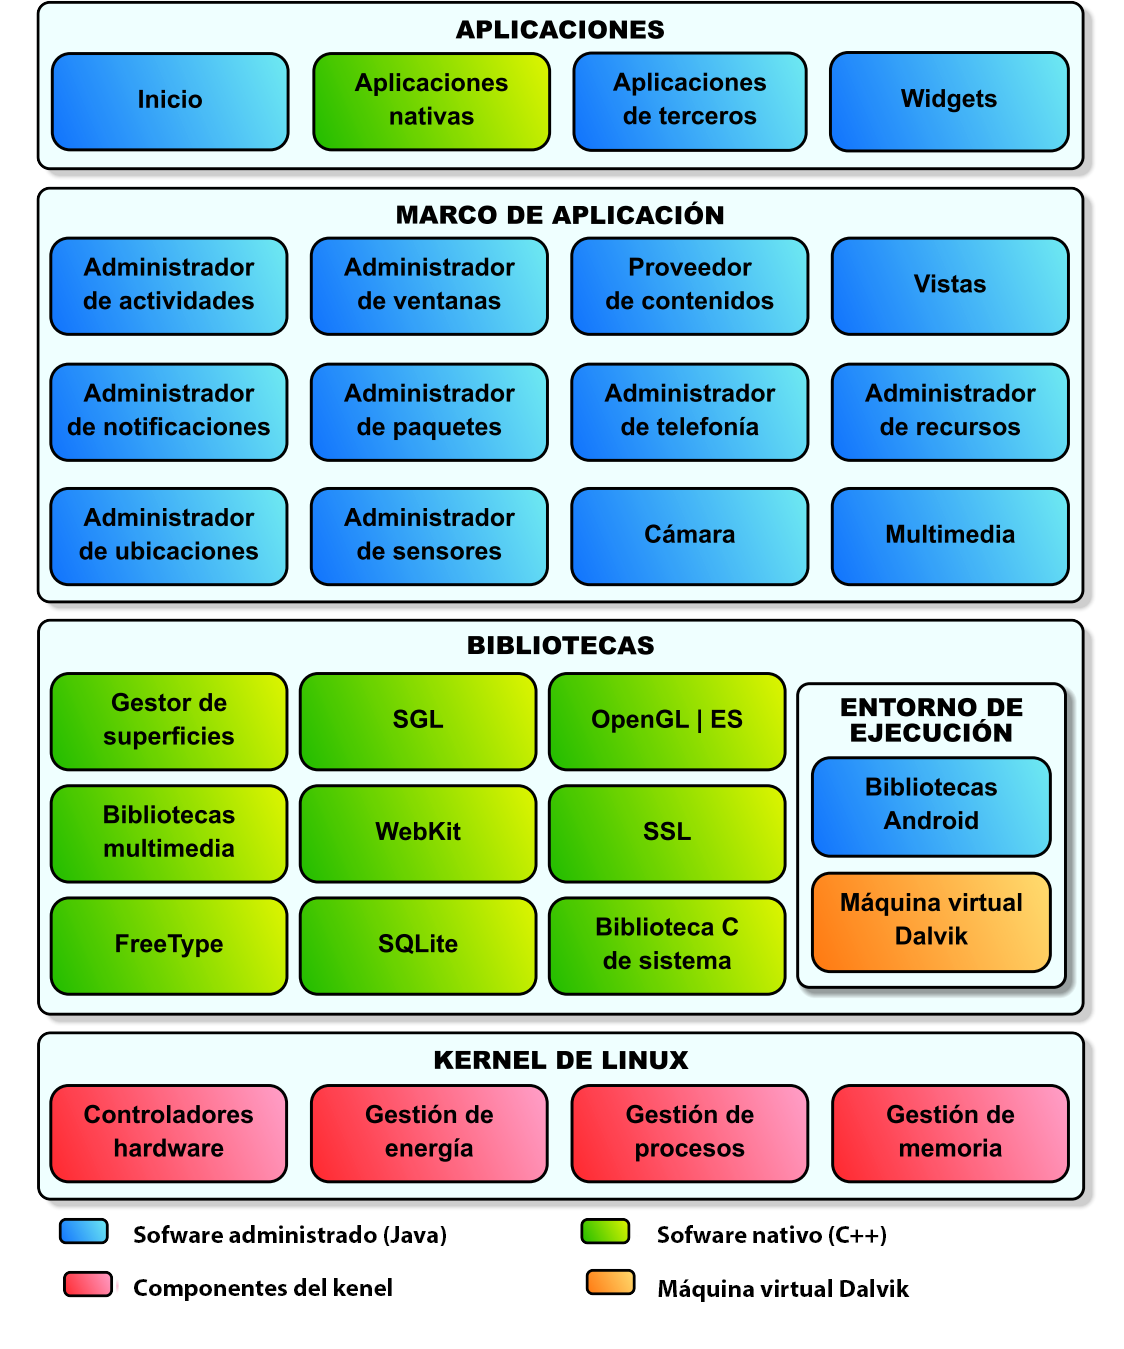
\includegraphics[scale=0.5]{imagenes/pila-android.png}
	\end{center}
	\caption{
		\label{fig:archi}
		Arquitectura del Sistema Operativo Android \cite{AAT}
	}
\end{figure}

\begin{itemize}
\item Aplicaciones: En este nivel se encuentran todas las aplicaciones presentes en el equipo, tanto las instaladas por el usuario como las provistas por el fabricante. Es importante destacar que todas cuentan con la misma capacidad para acceder los servicios que proporciona el sistema operativo. Gracias a esto, se pueden hacerse desarrollos que usen los mismos recursos que usan las aplicaciones nativas. \cite{AAT}.
\item Marco de aplicación: Esta capa esta formada por las diferentes clases que componen el \textit{API} que permiten a las aplicaciones realizar sus funciones, constituyen en el entorno de trabajo que posibilita acceder a los diferentes recursos del dispositivo \cite{AAT}.
\item Bibliotecas: Esta capa se ubica justo sobre el Kernel del sistema operativo y está constituida por un conjunto de bibliotecas escritas en \textit{C} o \textit{C++} que son compiladas para la arquitectura específica del equipo, su función es interactuar con el sistema operativo para acceder a los diferentes recursos gestionados por éste y poner al alcance de las aplicaciones la funcionalidad respectiva.\cite{AAT}. 
\item Entorno de ejecución: Este no se considera una capa como tal puesto que se compone principalmente de un conjunto de bibliotecas que proporcionan la funcionalidad base. El elemento principal de esta sección es la maquina virtual Dalvik que ejecuta cada de las aplicaciones instaladas en el dispositivo \cite{AAT}. 
\item Kernel de Linux: El núcleo del sistema operativo Android es un kernel Linux bastante similar al que puede incluir cualquier distribución de GNU/Linux conocida. En el caso de Android se realizan adaptaciones que permita ajustarse a las características del hardware en el que se ejecutará. Su función principal es proveer una capa de abstracción para el hardware y gestionar los diferentes recursos del teléfono y del sistema operativo \cite{AAT}.
\end{itemize}

\paragraph{Estructura básica de una aplicación Android}\mbox{}

Una actividad es una clase Java que contiene todo el código necesario para realizar una determinada tarea. Las actividades son el componente principal de las aplicaciones Android. Una aplicación puede estar compuestas por una o varias actividades que en conjunto desarrollan la funcionalidad de la aplicación. 

Por lo general, las actividades requieren la interacción del usuario. Para lograr esto, la actividad genera en la pantalla una serie de elementos, como campos de textos, botones, formularios, imágenes, entre otros. Estos elementos reciben el nombre de vistas, y son organizados y parametrizados mediante archivos \textit{XML} (\textit{Extensible Markup Language}) llamados \textit{layouts}. A pesar de que la disposición de las vistas es constantes en los archivos XML, una actividad puede modificar totalmente las vistas y sus atributos a tiempo de ejecución.

Cada vez que una aplicación ejecuta una actividad específica, se genera una pila con las actividades relacionadas. Es decir, solo una actividad puede estar en primer plano a la vez, las actividades predecesoras son empiladas en la memoria del teléfono. Cuando una actividad termina o el usuario presiona el botón atrás se pasa la siguiente en la pila. La figura \ref{fig:backstack} ilustra el comportamiento.

\begin{figure}[h]
	\begin{center}
		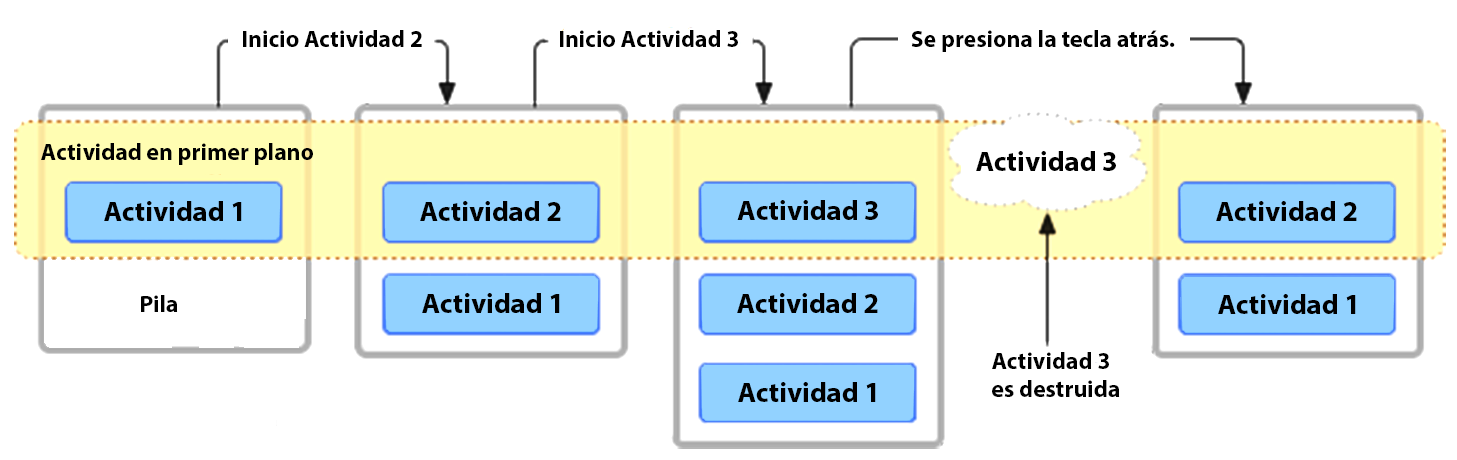
\includegraphics[scale=0.7]{imagenes/diagram_backstack.png}
	\end{center}
	\caption{
		\label{fig:backstack}
		Interacción y flujo de Actividades en Android \cite{TBS}
	}
\end{figure}

\paragraph{\textit{SQLite}} \mbox{}

\textit{SQLite} es un manejador de base de datos relacional de código abierto, usa sintaxis \textit{SQL} (\textit{Structured Query Language}), implementa transacciones y soporta \textit{triggers}, En \textit{SQLite} el conjunto de la base de datos (definiciones, tablas, índices, y los propios datos), son guardados como un sólo archivo y el requerimiento de memoria durante la ejecución es bastante bajo aprox 250KByte, lo que hace que este manejador sea fácilmente embebido en otros sistemas. Gracias a estas características el sitema Android cuenta con una base de datos \textit{SQLite} integrada y de fácil acceso para las aplicaciones.

\subsubsection{Eclipse}

Eclipse es un entorno integrado de desarrollo (\textit{Integrated development environment}, IDE por sus siglas en ingles) gratuito y de código abierto. Está escrito en \textit{Java} con el objetivo de realizar aplicaciones en este lenguaje. sin embargo permite la integración con otros como \textit{C, C++, Ada, Haskell, PHP, Python, Ruby}.

Este ambiente de trabajo es recomendado por Google para la construcción de aplicaciones Android, ya que a través de la instalación de un complemento distribuido en el sitio oficial, permite integrar en este entorno el soporte necesario para emplear diversas herramientas específicas para Android que facilitan el desarrollo. Cuenta con plantillas para las diversas clases básicas, instrumentos para el análisis del desempeño de la aplicación y facilidades para la gestión de emuladores que permiten simular \textit{smartphones} con diversas características y funciones.

Por ser el entorno oficial de desarrollo posee un amplio soporte y el respaldo de la comunidad, por lo que es el ambiente escogido para implementar Tuguia.de móvil.

\subsection{Tecnologías Asociadas con Tuguia.de} \label{subsect:Asociadas_movil}

Durante el desarrollo del proyecto, fue necesario incidir directamente sobre el API de Tuguia.de para agregar funcionalidad, hacer mejoras y ajustes necesarios para garantizar un adecuado desarrollo de la aplicación móvil, las tecnologías implicadas en este proceso serán descritas a continuación.

\subsubsection{Drupal}

Drupal es un marco de gestión de contenidos de código abierto escrito en lenguaje \textit{PHP}. En otra palabras, es una interfaz de programación de aplicaciones para crear sistema de gestión de contenidos (\textit{Content Managemement System}, CMS por su siglas en ingles). Una instalación base del sistema o \textit{el núcleo de Drupal} provee los elementos necesarios para el funcionamiento de un CMS básico, sin embargo, la funcionalidad se puede extender mediante la integración y desarrollo de módulos o paquetes\cite{TV10}.

El sitio Tuguia.de fue desarrollado con esta herramienta y mediante la instalación, configuración y elaboración de varios módulos fue implementado un API que permite mediante peticiones HTTP (\textit{Hypertext Transfer Protocol})gestionar el contenido del portal.

\subsubsection{Apache Solr} \label{subsubsect:solr}

Apache Solr es una plataforma de búsqueda de alto desempeño para sitios web, es de código abierto, esta escrita en lenguaje \textit{Java} y se basa en la biblioteca \textit{Apache Lucene} \cite{APS}. Apache Solr opera como un servicio separado del servidor web y la base de datos, puede incluso llegar a requerir un servidor dedicado para su operación. 

De forma sencilla el funcionamiento de Apache Solr puede ser descrito de la siguiente manera: Mediante archivos \textit{XML} llamados Documentos, se especifican los contenidos que serán indexados para su posterior búsqueda, estos índices pueden ser vistos como una lista de palabras en la que cada palabra en la lista posee una referencia hacia los elementos que la contienen, cuando se realiza una consulta a Apache Solr se ejecuta una búsqueda sobre las listas y se retornan los elementos que cumplan con el criterio establecido en la consulta.

Apache Solr permite realizar búsquedas de texto (\textit{Full-Text Search}) por palabra clave de forma similar al buscador de Google y tiene la capacidad para manejar búsquedas geoespaciales, por lo que en Tuguia.de, es ésta la herramienta elegida para realizar las búsquedas y es integrada a Drupal mediante un módulo de código abierto ampliamente configurable.  


% Marco Teorico.
\chapter{Marco Metodológico} \label{chap:marco_metodologico}

\vspace{5 mm}

En empresas TD es costumbre usar la metodología ágil Scrum, y los principios del desarrollo guiado por pruebas y comportamientos (\textit{Test-driven development y Behavior-driven development}), por lo tanto, el proceso de creación de la aplicación móvil para el portal \textit{Tuguia.de} estuvo enmarcado de ésta manera. En este capítulo se presenta y describe esta metodológia.
\section{Scrum} \label{sect:Scrum}

Scrum es un marco de trabajo iterativo e incremental para el desarrollo de proyectos y aplicaciones. El desarrollo esta organizado en ciclos de trabajo llamados \textit{Sprints} o iteraciones que son de duración fija y van sucediendo uno detrás de otro. Es importante destacar que sin importar que no se haya terminado el trabajo un \textit{Sprint} nunca se alarga \cite{DBLV09}. En el caso de Empresas TD las iteraciones tienen una duración de dos semanas.

\subsection{Roles en Scrum} 

Dentro de la metodología Scrum existen tres roles principales que debe ser cumplidos para la aplicación efectiva del proceso, estos son el el Dueño de Producto (DP), el Equipo y el ScrumMaster (SM). A continuación se describe cada rol, estas definiciones fueron extraídas de \cite{DBLV09}.

\begin{itemize}
\item El \textbf{Dueño del Producto} es el encargado de identificar las funcionalidades del producto y asignarles prioridad de acuerdo a las necesidades del negocio y debe revisar el resultado de cada iteración. Esta persona debe interactuar continuamente con el Equipo y tiene la autoridad final en el proyecto. En el caso de las pasantías el DP era el director general de Tuguia.de.
\item El \textbf{Equipo} es el encargado de construir el producto, en este caso el pasante. Debe poder autogestionarse y contar con un alto grado de autonomía y responsabilidad ya que al final de cada \textit{Sprint} debe poder tener un producto \textit{entregable}.
\item El \textbf{ScrumMaster} es el encargado de guiar al equipo y al DP en la aplicación y uso fructífero de Scrum, lo que hace es facilitar el proceso y ser un arbitro garante de la metológia y de que los demás actores ejecuten efectivamente su rol. Esta responsabilidad era de la gerencia e tecnología de Empresas TD.
\end{itemize} 

\subsection{El proceso de Scrum}

Como ya fue mencionado la metodología Scrum esta organizada en ciclos de trabajo que van ocurriendo uno tras otro. Estos ciclos están compuestos de actividades tal que se describe a continuación y como se muestra en la figura \ref{fig:scrum}. Las definiciones siguientes fueron obtenidas de \cite{DBLV09}.

\begin{figure}[h]
	\begin{center}
		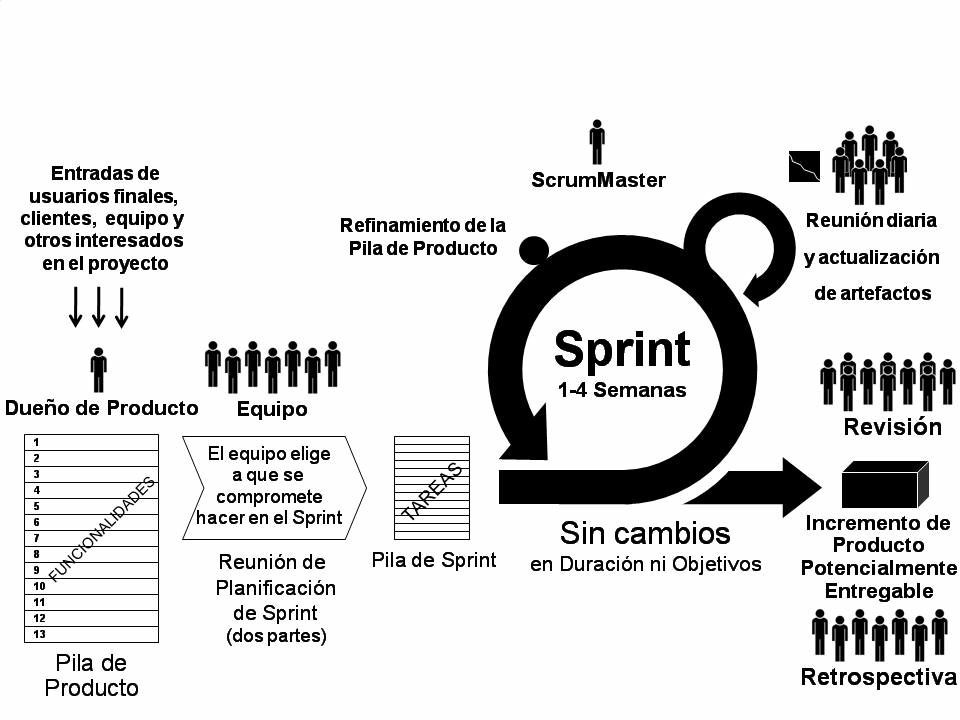
\includegraphics[scale=0.4]{imagenes/scrum.png}
	\end{center}
	\caption{
		\label{fig:scrum}
		Proceso Scrum \cite{DBLV09}
	}
\end{figure}

\begin{itemize}
\item \textbf{Planificación de la iteración:} La primera fase consiste en una reunión realizada al comienzo de la iteración donde al comienzo el DP presenta al equipo la lista de requisitos priorizada, se resuelven las dudas y se seleccionan los requisitos que se compromete a completar en la iteración, cada requisito es separado en tareas  yse estima la cantidad de esfuerzo en tiempo necesaria para completar cada una función del grado de dificultad de la misma.

\item \textbf{Ejecución de la iteración:} En esta fase más larga, en ésta se realiza el desarrollo del entregable. Durante esta fase, el equipo se reúne brevemente cada día para informar del progreso y dificultades. Cada miembro del equipo debe contestar únicamente las siguientes preguntas.
\begin{itemize}
\item ¿Qué ha hecho desde la última reunión?
\item ¿Qué tiene planificado hacer antes de la siguiente reunión?
\item ¿Qué impedimentos tiene o considera que va a tener?
\end{itemize}

\item \textbf{Inspección y adaptación:} Al finalizar el \textit{Sprint} se realiza una reunión, donde el equipo presenta el Dueño de la Aplicación los resultados obtenidos. En función de los resultados mostrados y de los cambios que haya habido en el contexto del proyecto, el DP realiza las adaptaciones necesarias de manera objetiva sobre la lista de requisitos. Por último el equipo debe analizar cómo ha sido su desempeño y cuales son los problemas que podrían impedirle progresar adecuadamente, tratando de mejorar de manera continua su productividad.

\end{itemize}








 

\section{Desarrollo Basado en Pruebas y Comportamientos} \label{sect:TDD_BDD}

El proceso de descrito por la metodología \textit{Scrum} no establece practicas especificas para la construcción del producto, es por esto que en Empresas TD se integran los principios del desarrollo Basado en Pruebas o \textit{Test Driven Development} (TDD)  y el Desarrollo Basado en Comportamientos, en inglés \textit{Behavior Driven Development} (BDD), como practicas a seguir durante el fase de programación. 

El procedimiento de desarrollo usando TDD se muestra en la figura \ref{img:tdd}.

\begin{figure}[h]
	\begin{center}
		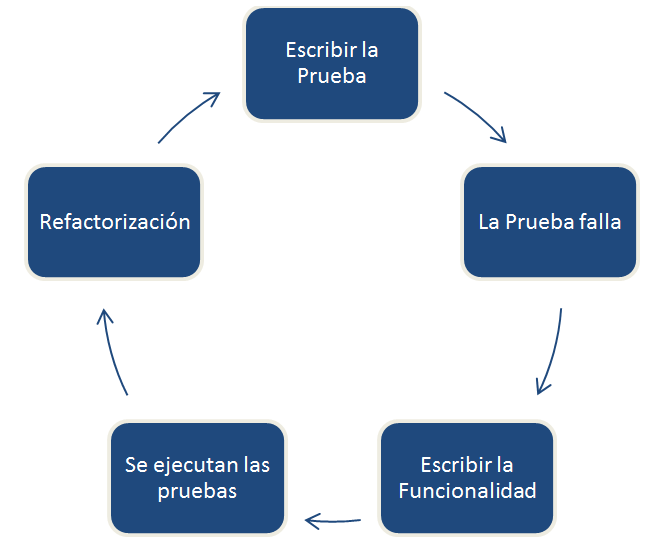
\includegraphics[scale=0.7]{imagenes/tdd.png}
	\end{center}
	\caption{
		\label{img:tdd}
		Ciclo de \textit{Test Driven Development}
	}
\end{figure}

En primer lugar, se escribe una prueba y se verifica que ésta falla. Luego se implementa el código que hace que la prueba pase satisfactoriamente y seguidamente se refactoriza el código escrito. Por último, se agrega una nueva prueba y se inicia el proceso nuevamente. Esta técnica es utilizada hasta que funcionalidad deseada este completa y funciona adecuadamente. 

La forma más efectiva de aplicar esta técnica es segmentar la funcionalidad en pequeñas unidades que puedan ser probadas de manera automatizada e inequívoca, de esta manera generar código simple y fácil de mantener gracias al proceso de refactorización asociado. Sin embargo aplicar esta técnica por sí sola es complejo, puesto que en ocasiones es difícil determinar qué probar y en qué nivel de detalle.

BDD surge como una manera de subsanar esta dificultad. En lugar basar las pruebas en pequeñas unidades de funcionalidad, BDD establece que las pruebas deben reflejar los comportamientos deseados por los diferentes actores involucrados en el proyecto. 

Para que se pueda aplicar BDD de manera adecuada es de vital importancia que todos los involucrados manejen un mismo léxico con respecto al proyecto, que les permita describir los comportamientos deseados en términos comunes sin caer en detalles de implementación. BDD sugiere la utilización de un formato similar al siguiente para especificar los comportamientos \cite{IBDD}.

Dado: Un contexto inicial.

Cuando: El evento a probar ocurre.

Entonces: Se aseguran que se alcancen los resultados deseados.

Este enfoque permite que las especificaciones no deban ser reescritas ya que el comportamiento pocas veces cambia durante el desarrollo, solo cambia la implementación. Además facilita el proceso de determinar los requerimientos mientras que acelera la documentación.



 



% DESARROLLO.
\chapter{Desarrollo del Proyecto} \label{chap:desarrollo}

\vspace{5 mm}

Este capítulo describe, el proceso de investigación, diseño, desarrollo e implementación del proyecto de pasantías. Se realiza una descripción del sistema actual y exponen las distintas tareas que conformaron las iteraciones de trabajo y se presentan los resultados obtenidos en cada una de ellas.


\section{Descripción del Sistema} \label{subsect:descripcion}
Antes de iniciar el con el desarrollo de la aplicación móvil se realizó un estudio de Tuguia.de con el objetivo familiarizarse con el contenido del sitio y el funcionamiento del API que alimenta la aplicación móvil.

\subsection{Contenido del Sitio}
El contenido de Tuguia.de es bastante variado, si bien el sitio esta planteado como una guía de locales, el portal no solo ofrece información sobre estos, también cuenta con contenido que corresponde a otro tipo de establecimientos y servicios, que van desde entidades financieras, instituciones gubernamentales, rutas de transporte, hasta  instituciones educativas. 

Los atributos relacionados con cada uno de estos \textit{nodos} de información es la siguiente: nombre, ciudad, urbanización, dirección, coordenadas geográficas, telefono de contacto, página web, correo electronico, cuenta en \textit{Facebook}, cuenta en \textit{Twitter} una o varias imagenes relacionadas, una puntuación que va del uno al cinco; esta puntuación es el resultado de promediar las calificaciones otorgadas por los usuarios en sus reseñas, por último, los nodos poseen una serie de taxonomías que permiten clasificarlos en diferentes categorías. 

Mediante la realización de peticiones de tipo HTTP en los servios provistos por el API es porsible gestionar los diferentes contenidos del sitio y sus atributos.

A continuación se presenta una imagen de un Local en Tuguia.de.

\begin{figure}[h]
	\begin{center}
		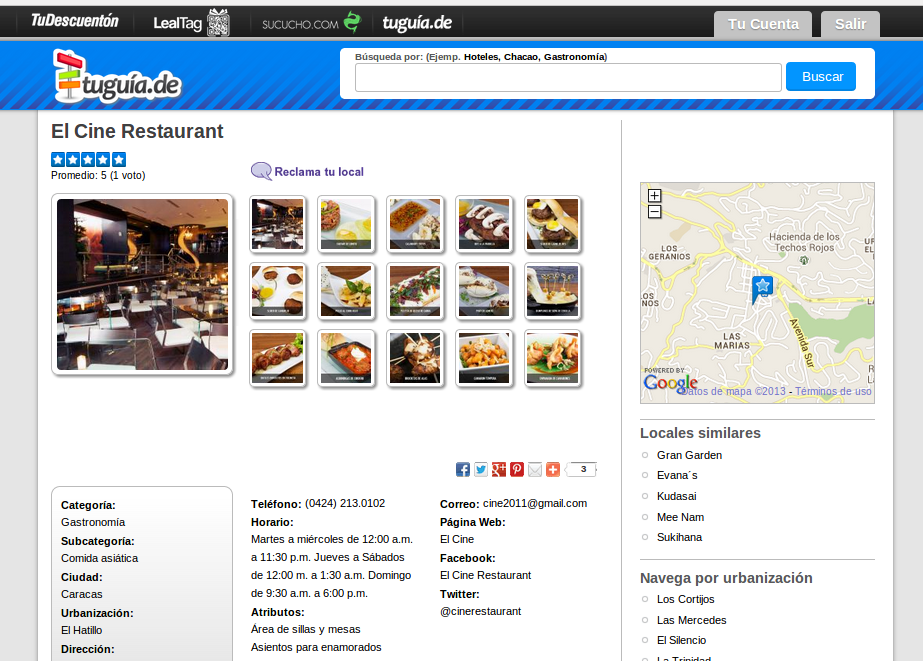
\includegraphics[scale=0.4]{imagenes/local_tgd.png}
	\end{center}
	\caption{
		\label{fig:localtgd}
		Local visto en Tuguia.de \cite{CTGD}
	}
\end{figure}



%\input{desarrollo/3_Solver_y_compilador.tex}
%\input{desarrollo/4_Implemetacion_y_resultados.tex}

%\input{conclusiones/conclusiones.tex}

% Crea el glosario 
\makeglossaries
%\printglossaries

% Establece las citas y bibliografia
\bibliographystyle{alpha.bst}
\bibliography{myrefs}

% Crea el apendice
\appendix
%\input{apendices/Archivos_intermedios.tex}
%\input{apendices/Ejemplos_del_lenguaje.tex}
%\input{apendices/Gramaticas.tex}

\printglossary

\end{document}
